\documentclass[11pt,a4paper]{article}
\usepackage[T1]{fontenc}
\usepackage{lmodern}
\usepackage{amsmath,amssymb}
\usepackage{graphicx,booktabs,tabularx}
\usepackage[margin=0.9in]{geometry}
\usepackage{microtype}
\usepackage[section]{placeins}
\usepackage[authoryear,round]{natbib}
\usepackage{hyperref}
\usepackage{xurl}
\hypersetup{colorlinks=true,linkcolor=blue,citecolor=blue,urlcolor=blue,
 pdftitle={Ranking Is Not Threshold Portability: Validating IFRS 16 Covenant Screening in a Synthetic Benchmark},pdfauthor={Aniket Bhardwaj}}
\graphicspath{{paper/figures/v3/}{figures/v3/}}
\IfFileExists{paper/generated/v3/values.tex}{\def\tablepath{paper/generated/v3/}}{\def\tablepath{generated/v3/}}
\newcommand{\exhibit}[1]{\input{\tablepath#1.tex}}
\newcommand{\val}[1]{\csname v#1\endcsname}
\exhibit{values}
\exhibit{provenance}
\setlength{\emergencystretch}{2em}
\setlength{\bibsep}{3pt}
\title{Ranking Is Not Threshold Portability:\\Validating IFRS 16 Covenant Screening\\in a Synthetic Benchmark}
\author{Aniket Bhardwaj\\\textit{Independent Researcher}\\\texttt{bhardwaj.aniket2002@gmail.com}}
\date{September 2026}
\begin{document}
\maketitle
\begin{abstract}
% Claims: SCR-001, SCR-002, SCR-003, SCR-004, SCR-006, SCR-007, SCR-008, SCR-012, SCR-014, SCR-015, ENG-001
Covenant screening requires separate validation of a mechanically consistent financial engine, a score that ranks adverse outcomes, and a decision threshold that transfers across borrower structures. We examine these layers in a synthetic IFRS 16 benchmark of \val{N} scenarios across five archetypes, including \val{Failures} broad financial failures. Archived independent checks and runtime invariants support the engine mechanics on the tested paths. The fixed screening score achieves ROC-AUC \val{AUC} and average precision \val{AP}. Leave-one-template-out thresholds selected only on the training archetypes raise recall from \val{FixedRecall} under the fixed 0.5 comparator to \val{TransferRecall}, but generate \val{TransferFP} false positives. This trade-off is sharply heterogeneous: Template 004 contributes 37 of 38 false positives, and its balanced accuracy is 0.513 under the transferred threshold versus 0.636 at 0.5. The score is not a calibrated probability of default, and sparse failures and overlapping training sets constrain inference beyond this synthetic realization. Strong ranking therefore did not imply threshold portability across synthetic borrower archetypes. Engine correctness, ranking performance, and decision usefulness require separate validation.
\end{abstract}
\noindent\textbf{Keywords:} IFRS 16; covenant screening; synthetic benchmark; threshold transfer; model validation.

% Architecture: S1
\section{Introduction}
% Literature: ifrs2016leases
IFRS 16 brings most lessee lease commitments onto the balance sheet, subject to the standard's exemptions \citep{ifrs2016leases}. In covenant screening, a lease-inclusive calculation and a stipulated rent-adjusted alternative need not represent the same contractual definition. The accounting convention therefore needs to be stated before interpreting a leverage or coverage test. Neither calculation, by itself, establishes the terms of an actual loan.

% Literature: nini2009creditor
The distinction between a covenant condition and a missed payment also matters for the interpretation of a screening outcome. The creditor-control perspective examined by \citet{nini2009creditor} motivates separating covenant conditions from debt-service events.

% Claims: SCR-001, SCR-002, SCR-015
This paper asks how much a successful validation result establishes about the next decision layer. A financial simulation may reconcile its cash and debt mechanics, while a screening score ranks its adverse outcomes well. Those findings do not establish that a threshold selected on one collection of structures will work on another. The question is not exhausted by the discrimination of the score: the usefulness of a threshold requires its own evaluation.

% Claims: SCR-001, SCR-002, SCR-016
The study is deliberately synthetic. Its contribution is a bounded demonstration of the distinction between mechanical correctness, ranking performance and threshold portability across stipulated borrower archetypes. It does not estimate borrower-population performance or claim that the observed transfer difficulty occurs with the same frequency outside this system. The central thesis is a possibility demonstrated within the benchmark: strong ranking can coexist with an unstable decision rule.

% Claims: SCR-002
The organization follows that distinction. We first establish what the mechanical validation supports, then separate the fixed score from the procedure used to select a threshold. Aggregate results are followed by the held-out template evidence, so that a favorable aggregate does not substitute for the examination of transfer. The limitations return to the scope of each validation layer.

% Architecture: S2
\section{Research question and contribution}
% Claims: SCR-001, SCR-002
The research question is whether a mechanically validated screening workflow with strong synthetic discrimination also supports a portable threshold across structurally different synthetic archetypes. The answer in this benchmark is qualified: ranking remains strong, but the transferred thresholds do not provide a stable rule across all the archetypes. This is the paper's primary conceptual result, rather than a claim of universal failure or universal success for screening models.

% Claims: SCR-002
Figure~\ref{fig:F1} distinguishes the three layers. Engine correctness concerns the consistency of the tested financial mechanics. Ranking performance concerns the ordering of adverse outcomes by the screening score. Decision usefulness concerns the behavior of the resulting threshold rule. Evidence at one layer must not be read as evidence that the next layer has passed. This distinction determines both the presentation of the results and the limits placed on their interpretation.

\begin{figure}[htbp]\centering
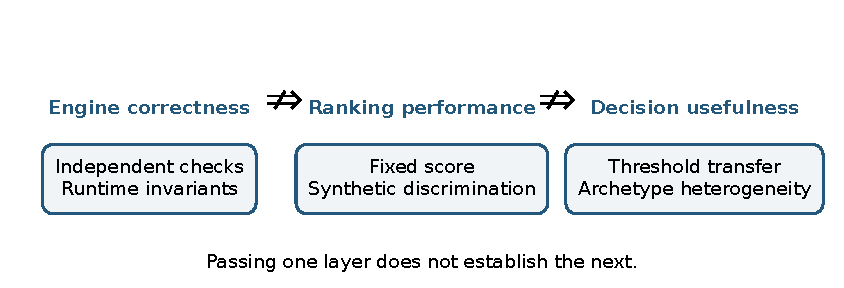
\includegraphics[width=\linewidth]{F1.pdf}
% Claims: SCR-001, SCR-002, ENG-001
\caption{Three distinct validation layers. Passing one layer does not establish the next. This is a conceptual synthesis of the frozen validation evidence, not a causal diagram or a claim about external borrower performance.}
\label{fig:F1}
\end{figure}

% Architecture: S2A
\section{Related literature and validation perspective}
% Literature: ifrs2016leases, dichev2002covenant, nini2009creditor, christensen2012covenants
Debt covenants turn accounting measurements into contractual control points. Large-sample evidence on accounting-based covenants shows that firms cluster close to covenant thresholds and that apparent technical violations are economically meaningful rather than rare accounting curiosities \citep{dichev2002covenant}. Covenant violations can transfer control rights to creditors and alter firm investment policy, which gives the measured boundary consequences beyond the label attached to a screen \citep{nini2009creditor}. Contract design also distinguishes capital covenants, which constrain balance-sheet positions, from performance covenants that act as trip wires when creditor claims become vulnerable \citep{christensen2012covenants}. These findings do not determine the contractual definition for a synthetic benchmark. They instead explain why the accounting convention, breach rule and tested financial mechanics must be explicit. IFRS 16 changes the recognition of most lessee obligations, subject to exemptions \citep{ifrs2016leases}; whether a credit agreement incorporates, freezes or adjusts that accounting treatment remains a separate contractual question. In the framework used here, this concern belongs first to engine correctness: a screen cannot be interpreted until the quantities entering it are calculated consistently with the stated convention.

% Literature: fawcett2006roc, hand2009auc, steyerberg2010performance
Ranking quality answers a different question. ROC analysis evaluates how a score orders positives and negatives as its threshold varies, and it is particularly useful when class frequencies or error costs make raw accuracy hard to interpret \citep{fawcett2006roc}. A high ROC-AUC can therefore support a discrimination statement without identifying a useful operating threshold. \citet{hand2009auc} goes further by showing that an AUC summary embeds assumptions about the relative costs of errors and can be misleading for comparison when those assumptions do not match the decision problem. The broader prediction-model literature likewise treats discrimination, calibration and decision-analytic value as separate dimensions of performance \citep{steyerberg2010performance}. That separation is central here. The screening score is a monotone ordering device derived from analytic headroom; it has not been calibrated as an event probability. Its AUC and average precision describe ranking within the frozen benchmark, while the confusion counts describe what happens after a particular decision rule is applied.

% Literature: vickers2006decision
Threshold choice adds an objective that ranking metrics do not supply. Decision-curve analysis formalizes this point by evaluating predictions through the relative consequences of false-positive and false-negative actions over candidate thresholds \citep{vickers2006decision}. That literature is developed for clinical decisions, but its narrow methodological lesson carries over: a threshold is useful only in relation to an action and the costs attached to the two kinds of error. Balanced accuracy gives equal weight to sensitivity and specificity and is a transparent selection objective for this experiment. It is not an estimate of economic utility. A transferred rule can improve aggregate balanced accuracy while imposing an unacceptable burden in one borrower structure, so threshold evaluation must retain both confusion counts and subgroup denominators.

% Literature: quinonero2008shift
Transport adds a third distinction. Dataset shift refers to changes in the joint distribution of inputs and outcomes between training and use, with covariate shift as the special case in which the input distribution changes \citep{quinonero2008shift}. The five archetypes in this study create a controlled form of structural heterogeneity rather than a sample from an identified borrower population. Leave-one-template-out evaluation asks whether a threshold chosen on four stipulated structures behaves similarly on the fifth. It is a stronger check of within-benchmark transfer than reapplying a threshold to its fitting rows, but it does not identify performance under an external population distribution. The overlapping training sets and sparse positive counts further limit any population-style interpretation.

% Literature: synthesis of cited covenant and validation sources
Together, these literatures motivate the paper's three layers. Accounting and covenant design define what the engine must compute; discrimination evidence evaluates the ordering produced by the score; threshold and transport evidence evaluates the resulting rule in its intended setting. This paper's narrower contribution is to use a synthetic IFRS 16 screening system to demonstrate why mechanical validation, discrimination and threshold portability should be assessed separately.

% Architecture: S3
\section{IFRS 16 covenant-screening setup}
% Claims: SCR-015, SCR-018
The outcome is broad financial failure over five annual observations. It is the union of nonpositive EBITDA, payment default, reserve funding deficit, leverage above 6.0, or interest coverage below 1.8. These are stipulated benchmark tests. Broad failure is consequently not interchangeable with payment default, and the covenant thresholds are not presented as the terms of observed loan contracts. Equality at a simulated covenant threshold is not a breach.

% Claims: SCR-018, SCR-007
Let $\mathrm{Lev}^{a}_{t}$ and $\mathrm{ICR}^{a}_{t}$ denote analytic leverage and interest coverage at the annual testing dates. The minimum analytic headroom and fixed screening score are
\begin{equation}
H^a=\min\left\{6.0-\max_t\mathrm{Lev}^{a}_{t},\ \min_t\mathrm{ICR}^{a}_{t}-1.8\right\},
\qquad z=\frac{1}{1+\exp(2H^a)}.
\label{eq:score}
\end{equation}
Classification declares a positive when $z\geq\tau$. The comparator uses $\tau=0.5$, including equality. The classification boundary and the strict simulated covenant-breach test therefore have different equality conventions.

% Claims: SCR-015, SCR-019
Throughout the paper, $z$ is called a screening score. It is not a calibrated probability of default. The analytic path and the financial simulation differ in timing, cash, financing and input conventions. Validation of the financial engine does not prove that the analytic path approximates the simulator within established error bounds. Nor can all cross-model differences be attributed to analytic approximation error alone. These distinctions constrain what can be inferred from agreement in rankings or disagreement in classifications.

\exhibit{T1}

% Architecture: S4
\section{Financial-engine mechanics and validation}
% Claims: ENG-001, ENG-003
The financial-engine checks provide a foundation for the subsequent screening evaluation. Independent geometric return and MOIC expectations match production within the recorded tolerance, and the independently derived debt schedule matches the production schedule. The checks address the reviewed implementation's financial mechanics; they are not comparisons with external transaction outcomes. Table~\ref{tab:T2} summarizes the archived evidence.

% Claims: ENG-002
All 1,000 benchmark scenario-years across 200 paths passed the recorded runtime invariants. The validation also detected six specified adversarial corruptions. The relevant invariants cover closing, cash, debt and roll-forward consistency on the tested paths. Deliberate corruption checks provide evidence that the validation detects the specified failures, rather than merely recording an uneventful execution.

% Claims: ENG-001, ENG-002, ENG-003
This evidence has a precise scope. It supports tested accounting and mechanical consistency and independent return/debt sanity checks. It is not proof of correctness for every possible input, economic validity for every modeling convention, or validation against real borrower transactions. The engine section is therefore a prerequisite to interpreting the synthetic exercise, not the paper's principal finding.
\exhibit{T2}

% Architecture: S5
\section{Synthetic benchmark and evaluation protocol}
% Claims: SCR-003, SCR-016
The screening benchmark contains \val{N} scenarios across \val{Templates} synthetic templates and \val{Failures} broad financial failures. Table~\ref{tab:T1} reports the stipulated archetype inputs. The hotel-archetype labels identify synthetic structures, not observations of named borrowers. Parameter percentages in the input table describe stipulated growth, margin or financing conventions; they are not estimated subgroup event frequencies.

% Claims: SCR-008
The score in Equation~\ref{eq:score} remains fixed. In each leave-one-template-out fold, the threshold is selected using only the other templates and then applied to the excluded template. The objective is maximum training balanced accuracy, the average of sensitivity and specificity. The frozen tie rule selects the lowest threshold within the stated tolerance of the maximum. Test scores and labels do not participate in threshold selection.

% Claims: SCR-008
The frozen candidates are the unique training scores, together with zero and the next representable value above one. The latter permits an all-negative classification even if a score equals one. The absolute tie tolerance is $10^{-12}$. These rules specify a threshold-selection procedure; they do not fit or recalibrate the screening score. The comparison uses the original fixed threshold alongside the training-selected threshold on the same held-out rows.

% Claims: SCR-008
Exclusion during threshold fitting is the relevant safeguard in this evaluation. It does not undo earlier choices in the construction of the synthetic benchmark, nor does it establish performance on new real operators. The experiment evaluates the transfer of the selected rule within the stipulated archetype system. It should not be described as validation of a learned borrower-default model.

% Architecture: S6
\section{Ranking performance versus threshold transfer}
\subsection{Strong discrimination of the fixed score}
% Claims: SCR-004, SCR-005
The screening score has aggregate ROC-AUC \val{AUC} and average precision \val{AP} on the \val{N} scenarios, of which \val{Failures} fail. Figure~\ref{fig:F2} displays the ROC and precision--recall curves from the frozen scores. Average precision is the reported precision--recall summary; it is not trapezoidal area under that curve. The result supports strong ranking within this synthetic benchmark.

% Claims: SCR-005
Aggregate held-out and pooled AUC are equal for a mechanical reason. The score is fixed and each original score--label pair appears once in the concatenated held-out rows. Excluding a template from threshold selection cannot change that aggregate ranking. The equality is therefore not an independent piece of evidence that discrimination transfers across templates. The new decision evidence is the behavior of the thresholds selected without the held-out template.

\begin{figure}[htbp]\centering
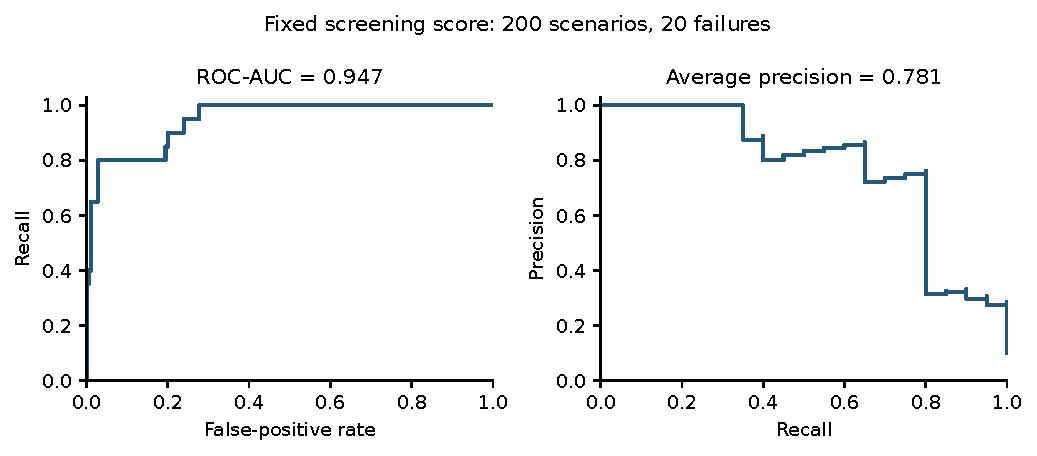
\includegraphics[width=\linewidth]{F2.pdf}
% Claims: SCR-003, SCR-004, SCR-005
\caption{Ranking of the fixed screening score on 200 scenarios, including 20 failures and 180 non-failures. The curves use frozen scores with ties grouped; no fitted curve, smoothing or confidence interval is added. The precision--recall annotation is average precision. Equality with the pooled AUC follows from unchanged score--label pairs and is not independent validation.}
\label{fig:F2}
\end{figure}

\subsection{Recall improves at a material false-positive cost}
% Claims: SCR-006, SCR-007
Table~\ref{tab:T3} gives the aggregate confusion counts. Training-selected thresholds yield \val{TransferTP} true positives, \val{TransferFP} false positives, \val{TransferTN} true negatives and \val{TransferFN} false negatives. The fixed comparator yields \val{FixedTP} true positives, \val{FixedFP} false positives, \val{FixedTN} true negatives and \val{FixedFN} false negatives. Both comparisons concern the same \val{N} held-out scenarios.

% Claims: SCR-006, SCR-007
Recall rises from \val{FixedRecall} under the fixed comparator to \val{TransferRecall} under transferred thresholds. Specificity falls from \val{FixedSpecificity} to \val{TransferSpecificity}. Balanced accuracy rises from \val{FixedBA} to \val{TransferBA}. The recall improvement must therefore be read together with the false-positive cost. Describing it simply as improved threshold performance would leave out a central part of the result.
\exhibit{T3}

% Claims: SCR-001, SCR-017
The aggregate comparison does not establish a portable decision rule. It also does not establish economic superiority: that would require an explicit error-cost or utility model. The question addressed here is narrower---whether the training-only rule behaves consistently across the held-out structures. That question requires the template-level evidence, even though the aggregate balanced-accuracy objective improves.

% Architecture: S7
\section{Held-out template results}
% Claims: SCR-009, SCR-010, SCR-011, SCR-012, SCR-013
Table~\ref{tab:T4} and Figure~\ref{fig:F3} make the uneven transfer visible. Template 001 misses four of its five failures among 38 scenarios. Template 002 detects all three failures and falsely flags one of its 29 non-failures among 32 scenarios. Template 003 misses its only failure among 47 scenarios despite within-template AUC 1.000. A ranking estimate based on a single positive cannot support a precise inference about broader performance.

% Claims: SCR-012
Template 004 contributes 37 of the 38 aggregate false positives. Its transferred threshold is 0.009678. Among its 49 scenarios, there are 11 failures and 38 non-failures; specificity is 2.6\% (1/38) and the false-positive rate is 97.4\% (37/38). Balanced accuracy is 0.513 under the transferred threshold, below 0.636 under the fixed comparator. This fold is the clearest example of aggregate improvement coexisting with poor local transfer.

% Claims: SCR-013, SCR-014
Template 005 contains no failures among 34 scenarios. Its within-template AUC, average precision and balanced accuracy are undefined under the frozen policy, rather than evidence of perfect ranking. More generally, fold dispersion is descriptive. Training sets overlap and positive counts are sparse in some templates. The aggregate is not an equal-weight average of template metrics and cannot replace the examination of these counts.
\exhibit{T4}

\begin{figure}[htbp]\centering
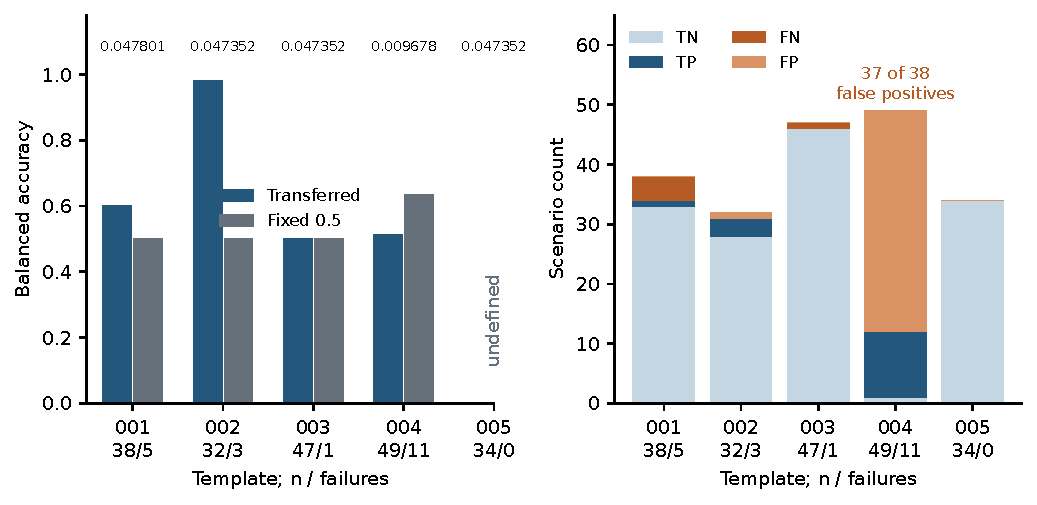
\includegraphics[width=\linewidth]{F3.pdf}
% Claims: SCR-009, SCR-010, SCR-011, SCR-012, SCR-013
\caption{Threshold-transfer heterogeneity. Left: transferred and fixed-threshold balanced accuracy, with selected thresholds annotated above; Template 005 is undefined. Right: transferred-threshold confusion counts, including the concentration of 37/38 aggregate false positives in Template 004. Tick labels show total scenarios/failures; non-failure counts follow from their difference. Aggregated classification is not an equal-weight average across templates.}
\label{fig:F3}
\end{figure}

\subsection{Cross-archetype heterogeneity}
% Claims: HET-001, HET-002, HET-009
The secondary evidence is convergent and descriptive. Template 004 shows weak threshold transfer and comparatively weak financing-policy outcomes, providing evidence within the same synthetic system consistent with structural heterogeneity affecting downstream transfer. Its financing regime mix is 48/100 base, 31/100 downside and 21/100 distressed, close to the stipulated probabilities of 50\%, 30\% and 20\%. Weakness persists after conditioning on regime, so the mixture alone does not explain it. Detailed cells appear in Appendix~\ref{sec:repro}.

% Claims: HET-001, HET-009, HET-010
This is not independent replication, external validation, causal evidence or empirical borrower evidence. The financing comparison remains a methodological demonstration, and regime-conditioned cells are small. The descriptive comparison does not show strict dominance on every risk metric: base and downside broad-failure rates under selected policies tie at zero. Template 004 has the lowest absolute opening cash and the highest debt/EBITDA among the stipulated archetypes, but not the lowest cash/EBITDA. That distinction prevents an unsupported interpretation of the cash ratios.

% Architecture: S10
\section{Limitations}
% Claims: SCR-014, SCR-015, SCR-017, REP-002
The benchmark is a synthetic system with few archetypes and sparse failures in some folds. The overlapping training sets do not supply independent replications. The score is not a calibrated probability of default, and neither the ranking result nor the threshold comparison establishes economic utility. These limitations restrict the result to the tested setting; they are not qualifications that can be removed by reporting the aggregate AUC more precisely.

% Claims: SCR-014, REP-002
The uncertainty presentation is descriptive. No new confidence intervals, bootstrap results or significance tests are introduced. Subgroup rates are accompanied by their sample sizes or numerator/denominator, including the small regime-conditioned financing cells. Undefined metrics remain undefined. These reporting choices preserve the distinction between the observed realization and a claim about a population of borrower structures.

% Claims: HET-001
The heterogeneity synthesis has no causal identification and no independently replicated or external borrower evidence. The same archetype system appears in both decision procedures. Convergence within that system is informative descriptively, but it cannot identify which structural component causes the transfer difficulty or establish that the same mechanism operates in observed borrowers.

% Claims: OPT-001, OPT-007, OPT-004, OPT-005, OPT-006
The financing-design experiment is retained as a methodological demonstration with stipulated assumptions. Its pervasive boundary selection and fixed-rate sensitivity restrict interpretation. There is no leverage-dependent credit pricing or recovery process, and the simulation continues mechanically after default. Entry and exit retain an asymmetric lease-treatment convention. These features preclude treating the selected policies as a substantive financing recommendation.

% Claims: BAY-001, BAY-002, BAY-003
The Bayesian calibration experiment is excluded from the substantive results. Unverified calibration inputs and failed frozen technical and prior-sensitivity gates preclude posterior integration. This exclusion concerns the examined experiment and its evidence; it is not a general judgment that Bayesian methods are invalid. Neither appendix changes the central screening result or supplies external borrower validation.

% Architecture: S11
\section{Conclusion}
% Claims: SCR-001, SCR-002, SCR-004, ENG-001
The synthetic benchmark separates three validation questions that should not be collapsed into one. The reviewed engine passes the archived mechanical checks on tested paths. The fixed screening score ranks adverse outcomes strongly. Yet that ranking does not establish a stable, portable threshold across structurally different synthetic archetypes. Passing one validation layer does not imply passing the next.

% Claims: SCR-001, SCR-002, SCR-006, SCR-007, SCR-012, SCR-017
Training-only threshold selection improves aggregate recall at a false-positive cost, with pronounced template-level instability. The methodological implication is to evaluate decision thresholds explicitly under structural heterogeneity rather than infer their usefulness from discrimination alone. The conclusion is conditional on this synthetic system: it demonstrates neither successful deployment in real borrowers nor economic superiority of the selected rule.
\clearpage
\appendix
\setcounter{table}{0}\renewcommand{\thetable}{A\arabic{table}}
\setcounter{figure}{0}\renewcommand{\thefigure}{A\arabic{figure}}
\renewcommand{\theHtable}{appendix.\arabic{table}}
\renewcommand{\theHfigure}{appendix.\arabic{figure}}
% Architecture: S8
\section{Financing-design experiment: methodological demonstration only}\label{sec:financing}
% Claims: OPT-001, OPT-002, OPT-007
The financing-design experiment is retained as a methodological demonstration only. The reviewed screening benchmark is unsuitable for sponsor-return optimization because its entry valuation is revenue-based while exit valuation is EBITDA-based. The separate financing experiment uses EBITDA for both valuation bases. This consistency does not establish market calibration or remove the retained entry/exit lease-treatment limitation.

% Claims: OPT-010
The separate experiment uses 100 operating scenarios per template and a frozen common policy grid. Each fold selects on the other four templates, using the same operating paths for candidates and the reference policy. Feasibility requires training broad-failure and payment-default rates no greater than the same-path reference rates. The objective is the training median limited-liability annualized sponsor return. Held-out results do not revise the grid or selection rule.

% Claims: LIM-001
For raw engine exit equity $E$ and positive initial sponsor equity $S$, the predeclared analysis-layer convention is
\begin{equation}
P=\max(0,E),\qquad M=P/S,\qquad r=M^{1/5}-1.
\end{equation}
Here $P$ is sponsor exit proceeds, $M$ is MOIC and $r$ is annualized sponsor return. Zero recovery gives MOIC zero and $r=-1$, or $-100\%$. Raw engine equity remains unfloored. This is a limited-liability sponsor-return convention, not an unconstrained financial IRR or a solver-failure convention.

% Claims: OPT-003, OPT-004, OPT-010
Table~\ref{tab:T5} reports the methodological comparison. Across the same 500 held-out operating scenarios per policy, median annualized sponsor return is 1.10\% under the selected policies and 0.61\% under the reference policies. Broad failure is 1.4\% (7/500) versus 6.8\% (34/500), and payment default is 0.6\% (3/500) versus 5.0\% (25/500). All five folds select the 1.50 debt/EBITDA lower boundary; four of five select the 70\% maximum sweep parameter.
\exhibit{T5}

% Claims: OPT-005, OPT-006, OPT-007, OPT-008
Figure~\ref{fig:A-F2} shows a systematic within-grid preference for lower leverage across the feasible observed debt levels. It does not establish what happens below the lower boundary or at infeasible levels. Fixed-rate sensitivity changes policy components in 2/5 folds. The independent known-optimum toy, training-only checks and runtime invariants support search mechanics, but do not establish economic optimality. Missing endogenous credit pricing and recovery, together with mechanical continuation after default, keep the outcome methodological.

\begin{figure}[htbp]\centering
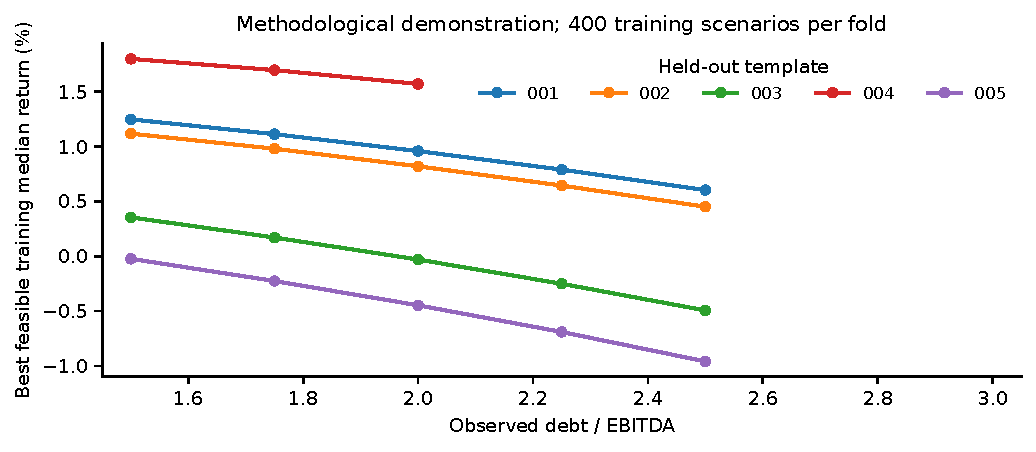
\includegraphics[width=\linewidth]{A-F2.pdf}
% Claims: OPT-004, OPT-005, OPT-010
\caption{Feasible observed debt-objective profile in the methodological financing demonstration. Each fold uses 400 training scenarios. Points are archived best-feasible objectives; infeasible levels are missing, and no curve extends below 1.50. Connecting observed feasible levels is a display aid, not an estimated surface. The within-grid pattern does not establish an economic optimum.}
\label{fig:A-F2}
\end{figure}

\clearpage
% Architecture: S9
\section{Excluded Bayesian calibration experiment}\label{sec:bayes}
% Claims: BAY-001, BAY-002, BAY-003
The Bayesian calibration experiment is excluded from the substantive results. The corrected experiment examined synthetic recovery, but the ten named-firm calibration rows remained unverified/stipulated. Firm names are not variable-level provenance. The recorded convergence/effective-sampling and prior-sensitivity gates did not support integration, and no posterior samples were used in the LBO results.

% Claims: BAY-003
Table~\ref{tab:A1} places the failed gates alongside the diagnostic evidence. Attractive synthetic recovery does not overcome poor provenance and failed admission criteria. The relevant methodological conclusion is exclusion of this experiment from substantive results, not an empirical calibration finding. A recovery exercise with stipulated inputs cannot supply the missing evidentiary basis for those inputs.

% Claims: BAY-001
This decision does not imply that Bayesian population modeling is intrinsically invalid. It bounds what the current evidence permits. The exclusion is preserved here because it limits the admissible interpretation of the broader workflow, not because the excluded method is a principal contribution of the paper.
\exhibit{A1}

\clearpage
% Architecture: S12
\section{Regime diagnostics and reproducibility}\label{sec:repro}
\subsection{Small-cell financing diagnostics}
% Claims: HET-003, HET-004, HET-005, HET-006, HET-007, HET-008, HET-009
Table~\ref{tab:A2} reports the Template 004 regime cells and the selected-policy median-return comparison across templates. The numbers are descriptive outcomes from the same synthetic system. The cell counts appear beside all return percentages, and event rates show counts and denominators. Figure~\ref{fig:A-F3} presents the within-regime comparison without confidence bars. Template 004's selected-policy median return is the lowest among the templates in each regime, while some risk metrics tie.

% Claims: HET-005, HET-008
In the distressed cell, $n=21$. Selected policies yield broad failures 7/21 (33.3\%), payment defaults 3/21 (14.3\%), insolvencies 6/21 (28.6\%), covenant breaches 7/21 (33.3\%), and total equity loss 1/21 (4.8\%). Reference policies yield the respective counts 18/21 (85.7\%), 16/21 (76.2\%), 18/21 (85.7\%), 14/21 (66.7\%), and 7/21 (33.3\%). The small denominator is integral to the interpretation of each percentage.

% Claims: LIM-002
Template 004 reference distressed P10 annualized sponsor return is $-100\%$ ($n=21$). Seven of the 21 scenarios have zero recovery, so the 10th percentile lies on that zero-recovery mass. This is mechanically consistent with the predeclared limited-liability convention. It does not mean raw equity is bounded at $-100\%$, that an unconstrained IRR was calculated, or that a solver failed.
\exhibit{A2}

\begin{figure}[htbp]\centering
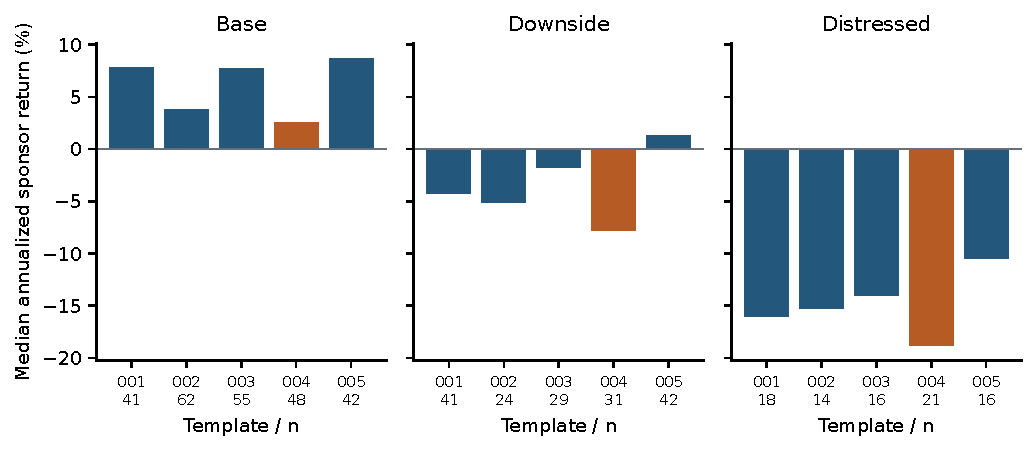
\includegraphics[width=\linewidth]{A-F3.pdf}
% Claims: HET-001, HET-009
\caption{Selected-policy median annualized sponsor return within each realized regime; tick labels show template and n. Template 004 is highlighted. The financing experiment remains methodological, and the comparison is descriptive within the same synthetic system, not independent replication or causal evidence. Distressed Template 004 has n=21. No uncertainty bars are inferred.}
\label{fig:A-F3}
\end{figure}

\subsection{Screening score distributions}
% Claims: SCR-004, SCR-009, SCR-010, SCR-011, SCR-012, SCR-013
Figure~\ref{fig:A-F1} displays the frozen screening scores directly by template and outcome. No density smoothing or score recalibration is used. The transferred threshold is shown for each template, with total and positive counts retained. The display supports the ranking-versus-threshold distinction without treating a score value as an estimated default probability.

\begin{figure}[htbp]\centering
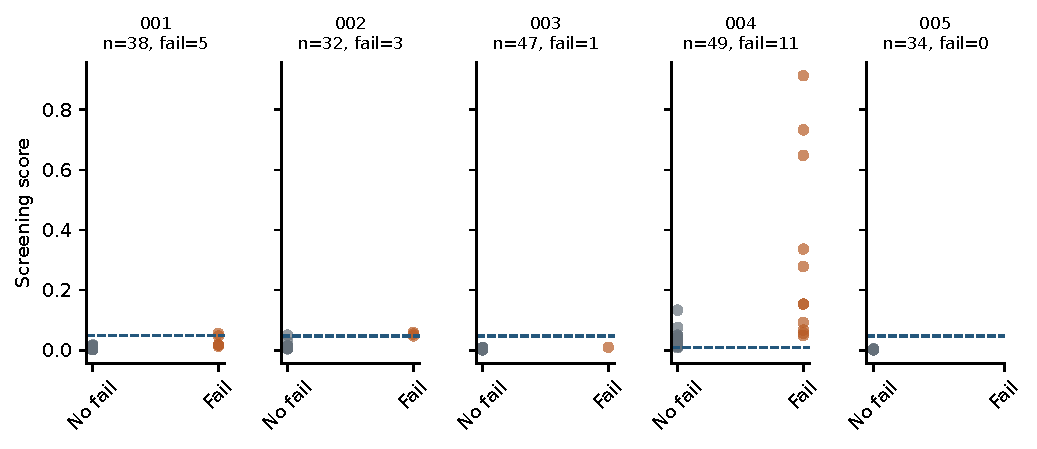
\includegraphics[width=\linewidth]{A-F1.pdf}
% Claims: SCR-004, SCR-009, SCR-010, SCR-011, SCR-012, SCR-013
\caption{Raw screening scores by template and failure status. Titles give n and failure counts; non-failure counts are the difference. Dashed lines mark transferred thresholds. Overlapping points retain their original values; no smoothing or uncertainty intervals are added. The single positive in Template 003 and absence of positives in Template 005 restrict within-template ranking inference.}
\label{fig:A-F1}
\end{figure}

\subsection{Artifact lineage and rendering}
% Claims: REP-001
The archived baseline reproduced its financial and statistical fields exactly, excluding runtime timing and source-commit metadata. Repository reproducibility does not establish external validity. The present manuscript uses frozen numerical outputs and adds only rendering, exposition and build verification.

% Reproducibility: source commits, paths, commands and seeds recorded in repository artifacts.
The claim-freeze commit is \texttt{21d726606f3208bcee6e3e84ae4c357e3a33d79b}; the manuscript source commit is \texttt{\buildsource}. The corrected pre-freeze source is \texttt{0f521a28150fe56f98cdabb3d1cb3664286df124}. Input and artifact hashes are preserved in the freeze source manifest, with protocol lineage in the freeze summary. Synthetic input definitions reside in \path{data/synthetic/operators.csv}. The screening benchmark uses seed 42; the separate financing demonstration uses seed 314159. These identify archived realizations and are not new simulation runs.

% Reproducibility: commands for rendering/building only, not model evaluation.
The rendering and PDF build commands are:
\begin{quote}\small\ttfamily
python -m analysis.scripts.render\_manuscript\_v3\\
python -m analysis.scripts.build\_manuscript\_v3
\end{quote}
The renderer reads the frozen specifications and source artifacts. The build uses Tectonic, the toolchain documented for the prior manuscript. Rendering records individual numeric fields and transformations; source comments retain claim links without exposing claim identifiers in the PDF. The final build audit records source and PDF hashes, exhibit counts, citation/reference checks and protected-artifact verification.

\subsection{Code and data availability}
% Reproducibility: public repository and exact manuscript lineage.
Code, synthetic inputs, frozen validation artifacts and reproduction instructions are available in the accompanying public repository at \url{https://github.com/Aniket2002/ifrs16-lbo-engine}. The repository branch \texttt{v3/validated-rebuild} contains the manuscript lineage; the exact manuscript-source commit is recorded above and in the build audit. No archival DOI is claimed.

\FloatBarrier
\begin{thebibliography}{9}
\bibitem[IFRS Foundation(2016)]{ifrs2016leases}
IFRS Foundation (2016). \emph{IFRS 16: Leases.}
International Accounting Standards Board.
\url{https://www.ifrs.org/issued-standards/list-of-standards/ifrs-16-leases/}.
\bibitem[Nini et~al.(2009)]{nini2009creditor}
Nini, G., Smith, D.~C., and Sufi, A. (2009).
Creditor control rights and firm investment policy.
\emph{Journal of Financial Economics}, 92(3), 400--420.
\url{https://doi.org/10.1016/j.jfineco.2008.04.008}.
\bibitem[Dichev and Skinner(2002)]{dichev2002covenant}
Dichev, I.~D., and Skinner, D.~J. (2002).
Large-sample evidence on the debt covenant hypothesis.
\emph{Journal of Accounting Research}, 40(4), 1091--1123.
\url{https://doi.org/10.1111/1475-679X.00083}.
\bibitem[Christensen and Nikolaev(2012)]{christensen2012covenants}
Christensen, H.~B., and Nikolaev, V.~V. (2012).
Capital versus performance covenants in debt contracts.
\emph{Journal of Accounting Research}, 50(1), 75--116.
\url{https://doi.org/10.1111/j.1475-679X.2011.00432.x}.
\bibitem[Fawcett(2006)]{fawcett2006roc}
Fawcett, T. (2006).
An introduction to ROC analysis.
\emph{Pattern Recognition Letters}, 27(8), 861--874.
\url{https://doi.org/10.1016/j.patrec.2005.10.010}.
\bibitem[Hand(2009)]{hand2009auc}
Hand, D.~J. (2009).
Measuring classifier performance: A coherent alternative to the area under the ROC curve.
\emph{Machine Learning}, 77, 103--123.
\url{https://doi.org/10.1007/s10994-009-5119-5}.
\bibitem[Steyerberg et~al.(2010)]{steyerberg2010performance}
Steyerberg, E.~W., Vickers, A.~J., Cook, N.~R., Gerds, T., Gonen, M., Obuchowski, N., Pencina, M.~J., and Kattan, M.~W. (2010).
Assessing the performance of prediction models: A framework for traditional and novel measures.
\emph{Epidemiology}, 21(1), 128--138.
\url{https://doi.org/10.1097/EDE.0b013e3181c30fb2}.
\bibitem[Vickers and Elkin(2006)]{vickers2006decision}
Vickers, A.~J., and Elkin, E.~B. (2006).
Decision curve analysis: A novel method for evaluating prediction models.
\emph{Medical Decision Making}, 26(6), 565--574.
\url{https://doi.org/10.1177/0272989X06295361}.
\bibitem[Qui\~nonero-Candela et~al.(2008)]{quinonero2008shift}
Qui\~nonero-Candela, J., Sugiyama, M., Schwaighofer, A., and Lawrence, N.~D., eds. (2008).
\emph{Dataset Shift in Machine Learning}.
MIT Press. ISBN 978-0-262-17005-5.
\url{https://mitpress.mit.edu/9780262545877/dataset-shift-in-machine-learning/}.
\end{thebibliography}
\end{document}
